\chapter{An efficient strategy for the collection and storage of petabytes of data for computation} \label{data-pipe}

%\section{Motivations} \label{Motivations}

\section{Abstract} \label{pipe-abstract}
In recent years, there has been an increasing amount of data being produced and stored, which is known as Big Data. The social networks, internet of things, scientific experiments and commercial services play a significant role in generating a vast amount of data. Three main factors are important in Big Data; Volume, Velocity and Variety. One needs to consider all three factors when designing a platform to support Big Data. A scientific experiment such as the Large Hadron Collider (LHC) is a data-intensive experiment, which is estimated to produce a volume of about 30 petabytes of data, annually. The velocity of these data that are propagated will be extremely fast. Traditional methods of collecting, storing and analysing data have become insufficient in managing the rapidly growing volume of data. Therefore, it is essential to have an efficient strategy to capture these data as they are produced. In this paper, a number of models are explored to understand what is the best approach for collecting and storing Big Data for analytics. Also, performance measurement of full execution cycles of these approaches on the monitoring of the Worldwide LHC Computing Grid (WLCG) infrastructure for collecting, storing and analysing is presented. Moreover, the models discussed are applied to a community driven software solution, Apache Flume, to show how they can be integrated, seamlessly.


%\linenumbers

\section{Introduction} \label{lbl-intro}
The field of data science has become a widly discussed topic in recent years due to a data explosion, especially with scientific experiments such as the Large Hadron Collider (LHC) at CERN and commercial businesses keen to enhance their competitiveness by learning about their customers to provide tailor made products and services, dramatically increasing the usage of sensor devices. The challenge of handling big volumes of data has been taken on by many companies, particularly those in the Internet domain, leading to a full paradigm shift in methods of data archiving, processing and visualisation. A number of new technologies have appeared, each one targeting specific aspects of big-scale distributed data-processing. All these technologies, such as batch computation systems (e.g. Hadoop) and non-structured databases (e.g MongoDB), can handle very large data volumes with little finacial cost. Hence, it becomes necessary to have a good understanding of the currently available technologies to develop a framework which can support efficient data collection, storage and analytics.

The core objectives of the presented study were the following:
\begin{itemize}
  \item Propose and design efficient approaches for collecting and storing data for analytics that can also be integrated with other data pipelines seamlessly.
  \item Implement and test the performance of the approaches to evaluate their design.
\end{itemize}

\section{Background} \label{lbl-review}
Over the past several years there has been a tremendous increase in the amount of data being transferred between Internet users. Escalating usage of streaming multimedia and other Internet based applications has contributed to this surge in data transmissions. Another facet of the increase is due to the expansion of Big Data, which refers to data sets that are many orders of magnitude larger than the standard files transmitted via the Internet. Big Data can range in size from hundreds of gigabytes to petabytes \cite{Verki1}.

Within the past decade, everything from banking transactions to medical history has migrated to digital storage. This change from physical documents to digital files has necessitated the creation of large data sets and consequently the transfer of large amounts of data. There is no sign that the continued increase in the amount of data being stored and transmitted by users is slowing down. Every year average Internet users are moving more and more data through their Internet connections. With the growth of Internet based applications, cloud computing, and data mining, the amount of data being stored in distributed systems around the world is growing rapidly. Depending on the bandwidth of these connections and the size of the data sets being transmitted, the duration of transfers could potentially be measured in days or even weeks. There exists a need for an efficient transfer technique that can move large amounts of data quickly and easily without impacting other users or applications \cite{Verki1}.

In addition to corporate and commercial data sets, academic data are also being produced in similarly large quantities \cite{Aamnitchi2}. To give an example of the size of the data sets utilised by some scientific research experiments, a recent study observed a particle physics experiment (DZero) taking place at the Fermi Lab research center. While observing the DZero experiment between January 2013 and May 2015, Aamnitchi et al. \cite{Aamnitchi2} analysed the data usage patterns of users. They found that 561 users processed more than 5 petabytes of data with 13 million file accesses to more than 1.3 million distinct data files. An individual file was requested by at most 45 different users during the entire analysed time period (2013 to 2015).

In the DZero experiment, and many like it, scientists are generating datasets with an extremely large number of data files. Use of entire datasets is quite popular amongst users, however the individual data files in these sets are rarely used concurrently since they are so numerous.

There are many scientific research initiatives that have similar data demands. The most popular example today is the LHC. This experiment is well known and thousands of researchers in the physics and computer science fields are involved. The four experiments being conducted at the LHC generate petabytes of data annually \cite{Minoli3, Nicholson4}. One experiment, ALICE, can generate data at the rate of 1.25 GB/s. Figure \ref{fig:lhc_data} illustrates the growth in the size of data sets being created and stored by CERN. This graph shows the total amount of storage (both disk and tape) utilised by all of the top-level servers in the CERN organisation. The amount of data stored in the system has grown at a steady pace over the past 3 years and is expected to grow faster now that the intensity of their experiments is increasing, which will result in more data collected per second \cite{LHC5}. 

Geographically dispersed researchers eagerly await access to the newest datasets as they become available. The task of providing and maintaining fast and efficient data access to these users is a major undertaking. Also, monitoring computing behaviours in the Worldwide LHC Computing Grid (WLCG), such as data transfer, data access, and job processing is crucial for efficient resource allocation. This requires the gathering of metadata, describes the data (e.g. transfer time), from geographically distributed sources and the processing of such information to extract the relevant value for the WLCG group \cite{Magnoni20}. Since the CERN experiments are so well known and many studies have been conducted on their demands and requirements, one can use the CERN LHC experiments as a suitable case study for this research.

To meet the computing demands of experiments like those at the LHC, a specialised distributed computing environment is needed. Grid computing fits the needs of the LHC experiments and other similar research initiatives.

\begin{figure}[H]
  \centering
  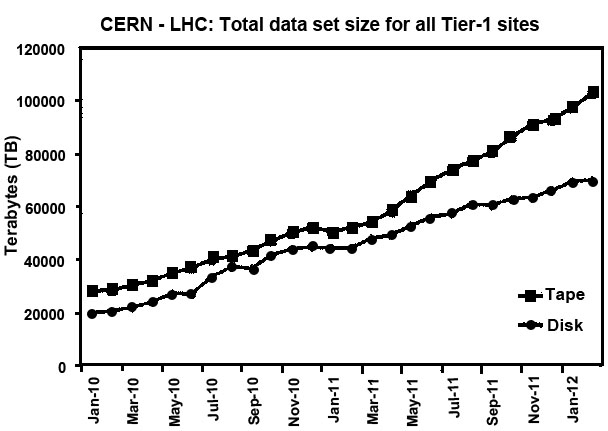
\includegraphics[width=100mm]{./Figures/lhc_data_size.jpg}
  \caption{\small Size of CERN LHC experimental data sets over the past years. The total disk and tape storage amounts aggregated for all Tier-1 locations in the CERN grid (adapted from \cite{LHC5}).}\label{fig:lhc_data}
\end{figure}

The Worldwide LHC Computing Grid (WLCG) was created by CERN in 2002 in order to facilitate the access and dissemination of experiment data. The goal of the WLCG is to develop, build, and maintain a distributed computing infrastructure for the storage and analysis of data from LHC experiments \cite{Knobloch6}. The WLCG is composed of over a hundred physical computing centers with more than 100,000 processors \cite{LHCGrid7}. Since the data sets produced by the LHC are extremely large and highly desired, the WLCG utilises replication to help meet the demands of users. Copies of raw, processed, and simulated data are made at several locations throughout the grid.

The WLCG utilises a four-tiered model for data dissemination. The original raw data is acquired and stored in the Tier-0 center at CERN. This data is then forwarded in a highly controlled fashion on dedicated network connections to all Tier-1 sites. There are eleven Tier-1 sites located in Canada, Germany, Spain, France, Italy, Nordic countries, Netherlands, Taipei, United Kingdom and USA.

The role of the Tier-1 sites varies according to the particular experiment, but in general they have the main responsibility for managing the permanent data storage - raw, simulated, and processed data - and providing computational capacity for processing and analysis \cite{Knobloch6}. The Tier-1 centers are connected with CERN through dedicated links (Figure \ref{fig:lhc_network}) to ensure high reliability and high-bandwidth data exchange, but they are also connected to many research networks and to the Internet \cite{LHCGrid7}. The underlying components of a Tier-1 site consist of online (disk) storage, archival (tape) storage, computing (process farms), and structured information (database) storage. Tier-1 sites are independently managed and have pledged specific levels of service to CERN. It is therefore left to the site’s administrators to guarantee that these services are reliably provided.

The Tier-2 sites are used for Monte Carlo event simulation and for end-user analysis. Any data generated at Tier-2 sites is forwarded back to Tier-1 centers for archival storage.

Other computing facilities in universities and laboratories are able to retrieve data from Tier-2 sites for personal processing and analysis. These sites constitute the Tier-3 centers, which are outside the scope of the controlled WLCG project and are individually maintained and governed. Tier-3 sites allow researchers to retrieve, host, and analyse specific datasets of interest. Freed from the reprocessing and simulation responsibilities of Tier-1 and Tier-2 centers, these Tier-3 sites can devote their resources to their own desired analyses and are allowed more flexibility with fewer constraints \cite{Grim8}. As there are thousands of researchers eagerly waiting for new data to analyse, many users will find less competition for time and resources at Tier-3 sites than at the Tier-2 sites.

It is important to note that users connecting to either Tier-2 or Tier-3 sites will use public, shared network connections, including the Internet. Grid traffic and normal World Wide Web traffic will both be present on these shared links. A user will also be sharing the site that they access with multiple other users. These factors can affect the performance of the data transfer between the selected retrieval site and the user. Retrieving these large data files also places a burden on shared resources and impacts other grid and non-grid users. When it comes to retrieving data in the WLCG, a normal user (depending on their security credentials) can access data on either Tier-2 and Tier-3 sites. The user would select a desired site and issue a request for a specific data file. Selecting a site to utilise can be a complicated task, with the performance a user obtains being dependent on the location chosen.

\begin{figure}[H]
  \centering
  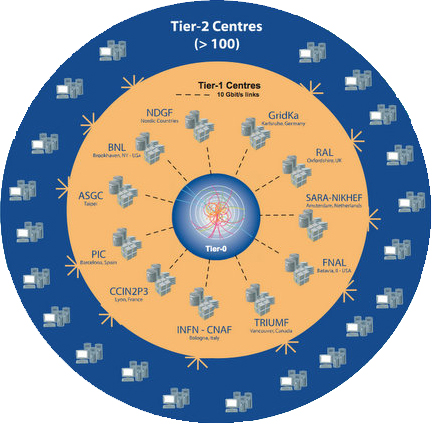
\includegraphics[width=100mm]{./Figures/lch_network.jpg}
  \caption{\small WLCG Tier-1 and Tier-2 connections \cite{LHCGrid7}.}\label{fig:lhc_network}
\end{figure}

Grid computing has emerged as a framework for aggregating geographically distributed, heterogeneous resources that enables secure and unified access to computing, storage and networking resources \cite{Foster9} for Big Data. Grid applications have vast datasets and/or complex computations that require secure resource sharing among geographically distributed systems. The term “grid” was inspired by the electrical grid system, where a user can plug in an appliance to a universal socket and have instant access to power without knowing exactly where that power was generated or how it came to reach the socket \cite{Foster9}.

The vision for grid computing was similar. A user could simply access as much computing power as required through a common interface without concern for who was providing the resources. Currently, grids have not yet reached that level of simplicity.

Grids offer coordinated resource sharing and problem solving in dynamic, multi-institutional virtual organisations \cite{Foster10}. A virtual organisation (VO) comprises a set of individuals and/or institutions having access to computers, software, data, and other resources for collaborative problem-solving or other purposes \cite{Laure11}. A grid can also be defined as a system that coordinates resources that are not subject to centralised control, using standard, open, general-purpose protocols and interfaces in order to deliver nontrivial qualities of service \cite{Foster12}. However, a number of new technologies have emerged for handling big-scale distributed data-processing, for example Hadoop, where the belief is that moving computation to where data reside is less time consuming than moving data to a different location for computation when dealing with Big Data. This is certainly true when the volume of data is very large because this approach will reduce network congestion and improve the overall performance of the system. However, a key grid principle contradicts with this as computing elements (CE) and storage elements (SE) in this scheme should be isolated. Currently, a lot of scientific experiments are beginning to adopt the ``new" Big Data technologies, in particular for metadata analytics at the LHC, hence the reason for the presented study.

Parallelising is used in order to enhance computations of Big Data. The well known MapReduce \cite{Dean13} framework that has been used in this paper has been well developed in the area of Big Data science and has the parallelisation feature. Its other features are its inherent data management and fault tolerant capabilities.

The Hadoop framework has also been employed in this paper. It is an open-source MapReduce software framework. For its functions it relies on the Hadoop Distributed File System (HDFS) \cite{Shvachko14}, which is a derivative of the Google File System (GFS) \cite{Ghemawat15}. In its function as a fault-tolerance and data management system, as the user provides data to the framework, the HDFS system splits and replicates input on some cluster nodes.

	The approaches for collecting and storing Big Data for analytics are applied on a community-driven software solution such as Apache Flume in this research in order to understand how it can be integrated seamlessly. Apache Flume is used for effectively gathering, aggregating, and transporting large amounts of data. It has a flexible and simple architecture, which makes it fault tolerant and robust with tunable and recovery mechanisms. It uses a simple extensible data model that allows online analytic applications \cite{Flume16}.

\section{Design and methodology} \label{lbl-dm}
When data messages are consumed from the transport layer and written into storage, there will most likely be some sort of data transformation carried out before storage in the storage layer. Such a transformation could be extracting the body from the message and removing the header as it is not required, or serialisation or compression. There needs to be a strategy in place to carry out the required transformation as this will play a significant role in improving the performance of subsequent computations. In this paper three different approaches were explored:

\begin{enumerate}
	\item Implement the data transformation logic within the data pipeline. Therefore, the messages, M, will be read by the consumer, to apply the transformation \(\langle\circlearrowright T\rangle \) and to write the results into the storage layer, S, for analytics \( \langle\circlearrowright A\rangle \):
	
		\centerline{\(M \xrightarrow[]{\langle\circlearrowright T\rangle}S\rightarrow  \langle\circlearrowright A\rangle \)}
		
	\item Write the raw messages, M, directly into storage layer, S, without any modification. Then there is another intermediate job \(\langle\circlearrowright iT\rangle\) that reads the raw data from storage, transforms the data and writes the results into a new path but to the same storage layer for analytics \( \langle\circlearrowright A\rangle \):
	
	\centerline{\(M\rightarrow S\xrightarrow {\langle\circlearrowright iT\rangle} S\rightarrow   \langle\circlearrowright A\rangle \)}
	
	\item Write the raw messages, M, into the storage layer, S, without any modification. Let the analytics \( \langle\circlearrowright A\rangle \) jobs carry out the transformation \(\langle\circlearrowright T\rangle \):
	
	\centerline{\(M \rightarrow S\rightarrow   \langle \langle\circlearrowright T\rangle +\langle\circlearrowright A\rangle \rangle \)}
	
\end{enumerate}

The first approach is the traditional way of transforming data. However, this relys too much on the data pipeline. If the data pipeline is replaced then the transformation logic would need to be reimplemented. Therefore, it is an inefficient design.

The second approach has two benefits as the transformation logic is moved to a centralised location and untampered raw data are stored as well as the transformed data. Therefore, in any case of inconsistency with the transformed data, it can be reconstructed from the raw data. This is not possible with the first method becasuse as soon as the data are transformed the raw data are discarded. Nevertheless, the second approach is very complex as there is a requirement for a job to transform the data and it raises the question of when and how this job should be scheduled. This approach also requires increased data storage as both raw and transformed data will be kept. A transformation job could be used here to compress the raw data and archive it to reduce the amount of storage required.

The third option is very simple and straight forward, as the raw data will be written into the storage layer without any modification. The transformation will only take place at the data analytics time. The transformation logic can be implemented in a shared library, which can be imported into any analytics jobs. Therefore, the transformation will take place as and when it is required. This way, the untempered raw data is still kept in the storage layer and no additional job or storage is needed for data transformation. Nonetheless, this method does add an extra execution time overhead to the analytics jobs and repetition of transformation. This should, however, not be too much of a problem as Big Data technologies are built to enhance computation speed by parallelising jobs. Hence, this arrangement should not significantly affect the execution time.

\subsection{Implementation} \label{lbl-implementation}
	The data pipeline presented in this paper uses Dirq library that offers a queue system using the underlying filesystem for storage for consuming messages, which allows concurrent read and write operations \cite{Dirg17}. Therefore, it can support a variety of heterogeneous applications and services that can write messages and have multiple readers reading the messages. The data pipeline was developed using the Hadoop native library that reads messages from the Dirq and writes them into HDFS using an appending mechanism. The Hadoop software framework was originally designed as create-once-read-many times system \cite{Hadoop18}. Therefore, appending was not available in the initial software release but later versions, 2.0 onwards, supported this mechanisum. Hadoop also has the benefit of working well with a few large files but is not so efficient when working with a large number of small files. The appending method is convenient as it allows for the creation of a single large file.

For the first approach, the data will be consumed from the Dirq, transformed and written into HDFS. The implementation of the second approach is similar to the first one with exception of no transformation. However, it requires chained MapReduce jobs in a centralised Hadoop cluster in order to take the raw data that has not previously been processed, and apply the appropriate data transformation, merge the transformed data with previously transformed data, delete the old transformed data, update the raw data as processed and merge and compress the raw data. An issue was encountered during testing of this appproach where it was found that data that were not processed by the transformation job were not available for analytics. The third approach is again like the second approach in that no transformation is carried out in the data pipeline, but the transformation logic is implemented in a common library and is available to be imported into any analytics jobs. Therefore, the transformation can be carried out as and when it is required. This approach will not have the issue of data unavailability as present in the other approaches as all written data will be picked up by the analytics jobs and the transformation will be done as and when required. All three approaches were implemented as a daemon that continuously ran on the CERN test infrastructure but will only check for data every 5 minutes, which causes a delay in making the data available for the analytics jobs.

In order to decrease the data aggregation delay from the data pipeline and to evaluate how easy it is to migrate to a different data pipeline, Apache Flume was used. Apache Flume is a community-driven software solution that receives messages from the transport layer and writes them into HDFS. There are three ways to flush consumed data into HDFS: periodically based on the elapsed time, the size of data or the number of events \cite{Flume16}. As expected, the first approach was complex as all the transformation logics were in the custom data pipeline so the transformation logics had to be reimplemented into Apache Flume. The second and third approach made the migration extremely simple, as all the transformation logics were implemented within the storage layer. But, as noted before, the second approach adds complexity to the storage layer, as it requires a chain of actions for data transformation. The third approach was the far simpler one, as no transformation was done at the Apache Flume side and no complexity of transformation was added at the storage layer. However, all three approaches encountered a common problem when Apache Flume pushes the events but does not flush the file until the configured file roll time is met, e.g. every 1 hour, the data being unavailable for computation during this time. While HDFS supports appending functionality, and the custom data pipeline, Apache Flume does not support it. The analytics jobs were able to read the data that were written by the custom data pipeline but not those written by Apache Flume. Therefore, the appending functionality was stripped out from the custom pipeline and implemented into Apache Flume, making it a custom library (see Algorithm~\ref{alg:append_alg}). With this amendment, Apache Flume was able to write a single file and append it while analytics jobs were able to read the data while the data were being written into HDFS.



\makeatletter
\def\BState{\State\hskip-\ALG@thistlm}
\makeatother


\begin{algorithm}[H]
\caption{File appending algorithm for Apache Flume: adding a close and reopen at every push to get the append behavior.}\label{alg:append_alg}
\begin{algorithmic}[1]
\Procedure{create-global-data-file-writer}{}
\State $ \text{declare a global DataFileWriter object}$
\State $ \text{create a file in HDFS}$
\State $ \text{initialise the file to global DataFileWriter}$
\item[]
\EndProcedure
\end{algorithmic}
\begin{algorithmic}[1]
\Procedure{consume-messages-and-sync-flush}{}
\State $ \text{create a temp  DataFileWriter refelecting(reopen) the global DataFileWriter}$
\State $ \text{consume all messages}$
\State $ \text{append mesages using temp DataFileWriter}$
\State $ \text{close temp DataFileWriter WHEN messages \( <=0 \)}$
\item[]
\EndProcedure
\end{algorithmic}
\begin{algorithmic}[1]
\Procedure{roll-files}{}
\State $ \text{close the global DataFileWriter} $
\item[]
\EndProcedure
\end{algorithmic}
\end{algorithm}


\section{Results and discussion} \label{lbl-results}
The three implementations discussed for this study were evaluated on the WLCG infrastructure that provides the computing resources to store, distribute and analyse the 30 petabytes of data, annually generated by the LHC and distributed around 150 computing centres around the world \cite{Gardner19}. LHC experiments utilise the XRootD protocol for data transfers and data access \cite{Gardner19}. This protocol is heavily used, hence the propagation of log messages is very intensive.

It is very complicated to carry out performance measurements on the three approaches, as they deploy different methods for consuming, writing and transforming the data. Therefore, in order to get a meaningful performance measurement, a full computation cycle was carried out; including consuming messages, writing to HDFS and carrying out a simple analytics job on those data. The full cycle was broken into three segments:

\begin{enumerate}[1.]
\item Data ingestion with data transformation and without data transformation.
\item Intermediate data transformation using a MapReduce job.
\item A simple statistical analytic computation using a MapReduce job with and without data transformation.
\end{enumerate}

In order to evaluate the proposed models, it was decided to push messages from the broker in batch sizes ranging from 10k to 100k. Data ingestion and analytics were conducted a few times for each batch of messages in order to capture an average performance time. The performance measurements were carried out on a heterogeneous Hadoop cluster that consisted of 15 nodes (8 nodes: 32 cores/64 GB, 7 nodes: 4 cores/8 GB).


\subsection{Performance results of data ingestion with and without data transformation} \label{lbl-perf-dpipe}
The first approach had to consume all messages from Dirq, apply a simple data transformation, which involved taking the source and destination IP address from the message and using a topology mapping file to determine the domain address and replace the IP address with the domain, and finally converting the data file into Avro format, which is a data serialisation framework that serialises the data into a compact binary format and writes the file into HDFS. As shown in Figure \ref{fig:pipe}, this approach (pre-trans-avro) is slower than the second approach (raw-json), which just reads the raw messages in JavaScript Object Notation (JSON), an easy-to-read format, and writes them into HDFS. The second approach is the fastest compared with the first and third approaches (raw-avro), which read raw data, convert them into Avro format and write them into HDFS. The third approach is faster then the first approach because it does not do any transformation.

\begin{figure}[H]
  \centering
  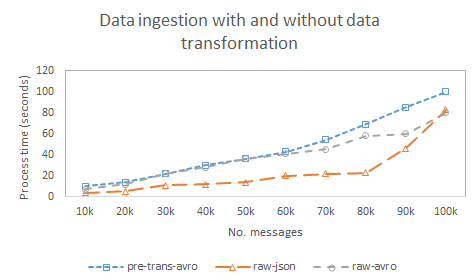
\includegraphics[width=100mm]{./Figures/datapipe_perf.jpg}
  \caption{\small Data ingestion from message queue to HDFS with and without data transformation.}\label{fig:pipe}
\end{figure}


Figure \ref{fig:ds} shows data representing unprocessed messages from the broker, raw JSON messages, a pre-transformed Avro and raw Avro file written into HDFS by the custom data pipeline. The Avro files are smaller than the JSON file and unprocessed data because they are serialised into binary format. However, the pre-transformed Avro file is larger than the raw Avro file because transformation was applied.

\begin{figure}[H]
  \centering
  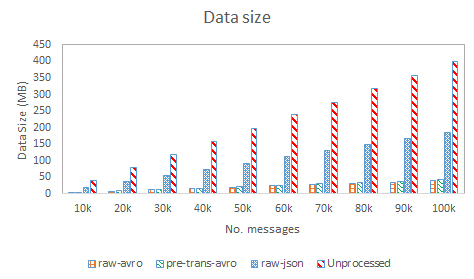
\includegraphics[width=100mm]{./Figures/data_size.jpg}
  \caption{\small Data size of the messages that were stored into HDFS with and without data transformation.}\label{fig:ds}
\end{figure}


\subsection{Performance results of intermediate data transformation using a MapReduce job} \label{lbl-perf-inter}
This test is designed to measure the performance of the intermediate transformation done on a centralised Hadoop cluster. As shown in Figure \ref{fig:mr_trans}, only the raw JSON data will go through this transformation, as the pre-transformed Avro file has already been transformed at the data pipeline level and the raw Avro data will be transformed at the analytic time when it is required. Transforming the data using an intermediate job is very expensive in terms of execution time, as they are chained MapReduce jobs that will transform, aggregate and merge the data. The majority of the overhead was used for finding resources and submitting the chained jobs to the Hadoop cluster.

\begin{figure}[H]
  \centering
  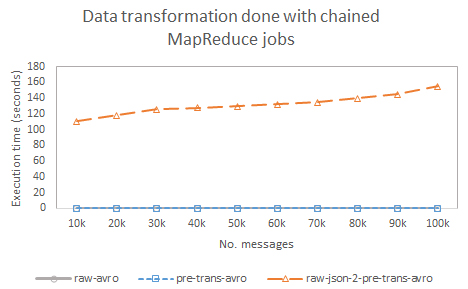
\includegraphics[width=100mm]{./Figures/mr_trans_perf.jpg}
  \caption{\small Intermediate MapReduce job for data transformation. Only the raw JSON messsages are transformed with the MapReduce job.}\label{fig:mr_trans}
\end{figure}

\subsection{Performance results of a simple analytic computation with and without data transformation} \label{lbl-perf-mr}
The final step of the evaluation cycle was to carry out a simple computation on the 100k messages dataset and measure the performance. Two sets of analytics jobs were implemented to compute a summary view of the XRootD operations, performed by the different users for each WLCG site belonging to the XRootD federation \cite{Gardner19}. An analytics job was modified to include the data transformation prior to the computation. The modified job was executed on the raw Avro data. As shown in Figure \ref{fig:mr_stats}, an extra overhead was added to the modified analytics job when compared with unmodified job that computed pre-transformed data, but the computation was seamless, as the MapReduce framework adopts a parallel programming model. Therefore, the jobs will be split into multiple tasks and will be sent to data nodes where the data reside.

\begin{figure}[H]
  \centering
  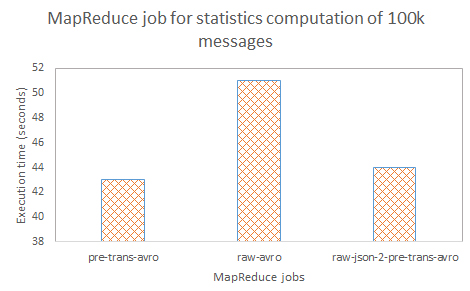
\includegraphics[width=100mm]{./Figures/mr_stats_perf.jpg}
  \caption{\small Performance measurements of the statistic computation were done on pre-transformed and the raw 100k dataset.}\label{fig:mr_stats}
\end{figure}

\subsection{Summary of the performance results} 
In order to understand which approach performed better, the execution time of the largest dataset of 100k messages was selected from Sections \ref{lbl-perf-dpipe}, \ref{lbl-perf-inter} and \ref{lbl-perf-mr} and the total is presented in Table \ref{table:tbresult}. It is clear that writing the raw Avro data into HDFS and letting the analytics do the transformation outperforms the other two approaches. The slowest seems to be the raw JSON file and having an intermediate job for transformation, which is understandable as they are chained jobs, which will add extra overheads. The pre-transformed Avro file by the data pipeline is not far from raw Avro data. But it will be beneficial to keep a copy of the untempered raw file in HDFS and let the analytics job do the transformation, which is better than pre-transformation as the authenticity is lost once the transformation is done and stored in HDFS.

\begin{table}[H]
\caption{Total sum of execution time for 100k dataset from Sections \ref{lbl-perf-dpipe} , \ref{lbl-perf-inter} and  \ref{lbl-perf-mr} are presented.}

\centering
    \begin{tabular}{ | l | l | l | l | l |}
    \hline 
 \multicolumn{1}{|p{2cm}|}{\centering \bfseries Transformation}
& \multicolumn{1}{|p{2cm}|}{\centering \bfseries Section \ref{lbl-perf-dpipe} \\ (secs)}
& \multicolumn{1}{|p{2cm}|}{\centering \bfseries Section \ref{lbl-perf-inter} \\ (secs)}
& \multicolumn{1}{|p{2cm}|}{\centering \bfseries Section \ref{lbl-perf-mr} \\ (sec)}
& \multicolumn{1}{|p{2cm}|}{\centering \bfseries Total \\ (secs)} \\\hline
    pre-trans-avro-mr & 100 & 0 & 43 & 143  \\ \hline
    raw-avro-mr & 80 & 0 & 51 & 131 \\ \hline
    raw-json-2-pre-trans-avro-mr & 83 & 155 & 44 & 282 \\ \hline
    \end{tabular}
		\label{table:tbresult}
\end{table}

%However, the is not much overhead to the data pipeline as it reads the messages and write the data into HDFS directly. Nevertheless, the data transformation and aggregation job is very expensive. In fact, it is extravagant than the first approach. %There is not additional overhead to data pipeline as same as the second approach but it does not have a separate complex job for data transformation. 



\subsection{Evaluation of Apache Flume} \label{lbl-flume}
There is still 5 minutes delay in polling data from the message queue. In order to eliminate the polling latency, the custom-made Apache Flume data collectors, as explained in \ref{lbl-implementation}, that utilise the appending mechanism were used. The performance test results shows that the third approach is optimal. Therefore, Apache Flume agents were configured to consume messages and flush them into HDFS directly. Figure \ref{fig:flum_stats} show spikes in the total number of messages propagated with a rate \( > \) 1 kHz, and it can be seen that Apache Flume seamlessly absorbs the load on its single virtual machine. Meanwhile, the old Oracle-based consumers used by WLCG, running on two production virtual machines, were struggling to keep up, causing a backlog of message stored in the broker.

\begin{figure}[H]
  \centering
  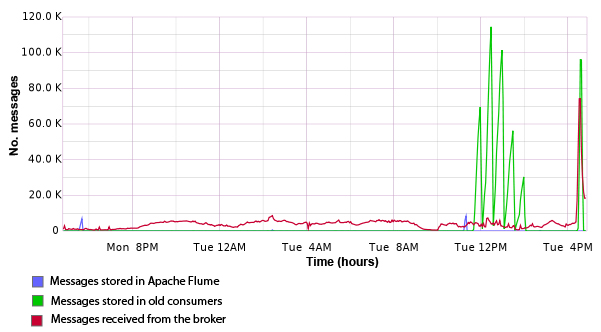
\includegraphics[width=100mm]{./Figures/flume_msg.jpg}
  \caption{\small Spikes of messages with a rate \( > \) 1 kHz. The red line is the messages received from the broker, green denotes the messages stored in old consumers, and blue denotes the messages stored in Apache Flume.}\label{fig:flum_stats}
\end{figure}


\section{Conclusion} \label{lbl-concl}
The approaches for consuming and storing data for analytics presented in this paper show how important it is to select the correct model for efficient performance and technology migration. It is clear from the study that keeping the main logic in a centralised location will simplify the technological and architectural migration. The performance test results show that eliminating any transformation at the data ingestion level and moving it to the analytics job is beneficial as the overall process time is reduced; untempered raw data are kept in the storage level for fault-tolerance, and the required transformation can be done with analytics jobs when required using a framework such as MapReduce. The WLCG group has adopted this approach, and it has been used for collecting, storing, and analysing metadata since April 2015 \cite{Magnoni20}. This approach can be easily applied to other use cases (e.g. business, for collecting customer interest datasets) and is not restricted to scientific applications.

%\section*{References}

%\bibliography{mybibfile}




